\section{The Cloud-Edge-Mobile Continuum}\label{sec:continuum}

\subsection{Definition}

Together, the computational resources from mobile, edge, and cloud computing have the potential of forming a \textit{continuum} on which new and disruptive types of applications can rely. Sometimes referred to as the Cloud-to-Things continuum, it enables the seamless convergence of infrastructure stretching from the cloud datacenter to devices on the network edge (including intermediate devices like ISP gateways, cellular base stations, and private cloud deployments) into a continuum of resources, to be provisioned to multiple tenants for hosting applications. Components of an application are hence able to run in a geo-distributed fashion using the services provided by the distributed infrastructure~\cite{GuptaIfogSim17}. 

%TODO: parts of this paragraph are unclear (e.g., interplay with the cloud properties?)
The key notion to bridge the gap in such a continuum is that of edge\footnote{In the literature the term ``edge'' is often used interchangeably with the term ``fog''.} computing, whose defining characteristics are edge location, dense geographical distribution, large-scale of deployment, support for mobility, resource and interface heterogeneity, and interplay with the cloud properties in order to address requirements of mobile applications that need low latency with a wide and dense geographical distribution~\cite{Bonomi2014}.  


%What: the challenges in materializing the continuum
\subsection{Key Characteristics and Challenges}

\begin{figure}[tbp]
	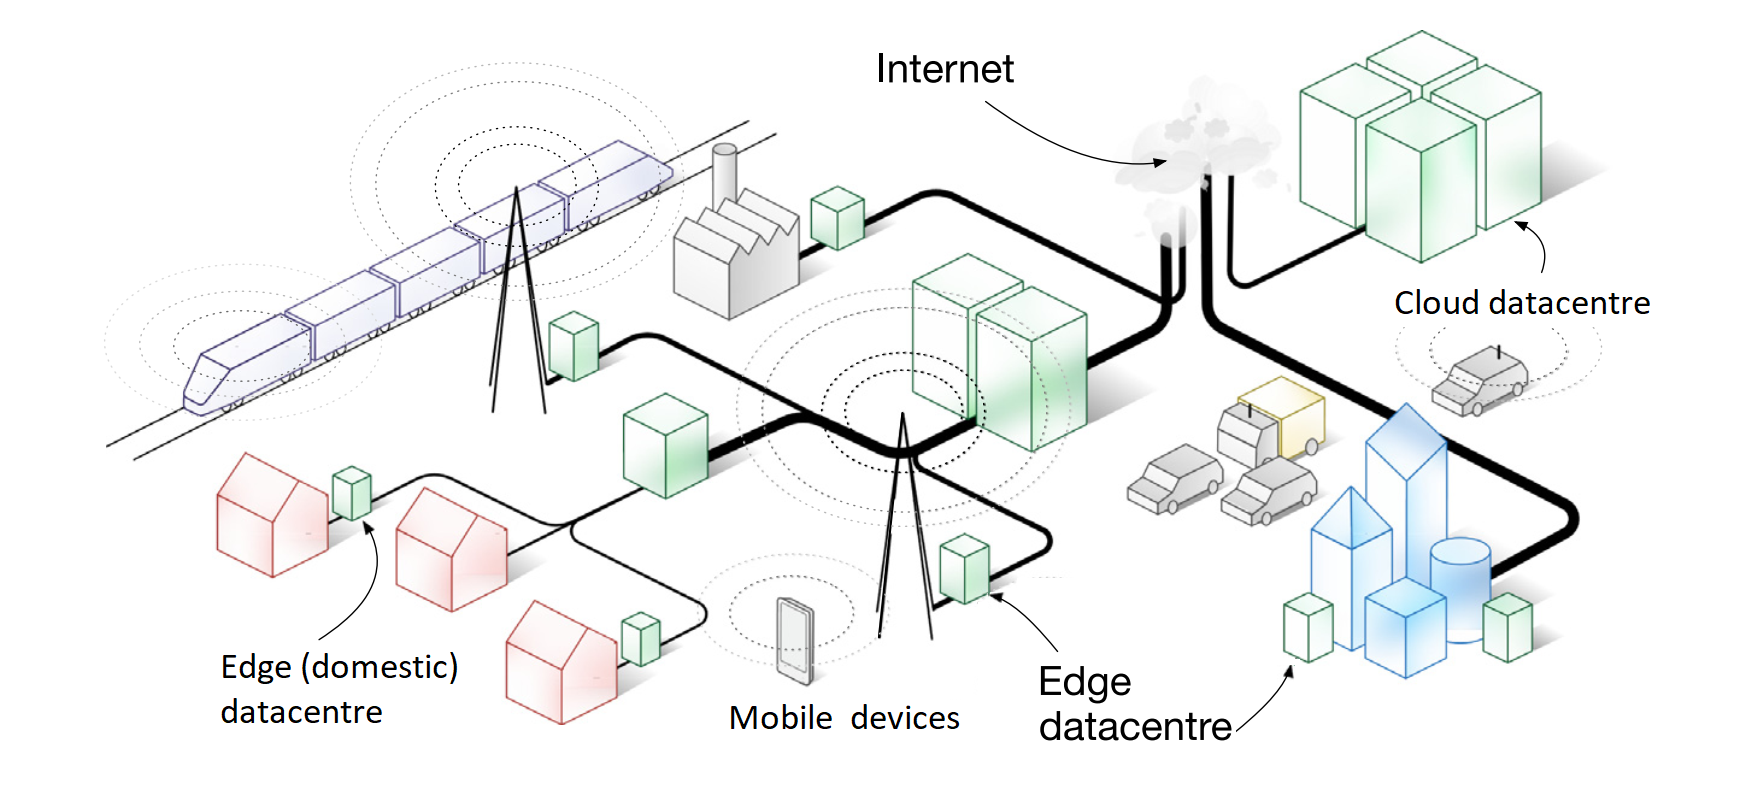
\includegraphics[width=0.9\textwidth]{figs/Continuum-overall.png}
	\caption{The computational continuum formed by coarsely distributed cloud datacenters, finely distributed edge datacenters, and mobile/IoT devices.}
	\label{fig:continuum-overral}
\end{figure}

\newcounter{req_count}
\newcounter{req_sub_count}[req_count]

%What: the challenge of heterogeneity; 
%\subsubsection{Heterogeneity}\label{sec:heterogeneity}

%\stepcounter{req_count}

The continuum encompasses heterogeneous types of computing platforms and technologies located at the cloud and at the edge of the network, as well as in mobile devices. Next, we identify the key characteristics of the cloud-edge-mobile continuum posing challenges to its realization along with the properties required to address these challenges.

%This heterogeneity poses challenges in terms of how each part of the continuum should allocate its resources to different types of client applications (provisioning) and how these applications should have access to the continuum resources (inter-operation). 

%In particular, 


%The realization of the continuum requires a flexible model that copes with this heterogeneity (Req. \stepcounter{req_sub_count}\textbf{R\arabic{req_count}.\arabic{req_sub_count}}).%, i.e., different instances of the model should address the many particularities in the continuum .
%, i.e., it should be agnostic with respect to the capabilities and specific technology details of different computing platforms and infrastructures in the continuum (Req. \stepcounter{req_sub_count}\textbf{R\arabic{req_count}.\arabic{req_sub_count}}); and 


%\begin{figure}[tbp]
%	\centering
%	\captionsetup[subfigure]{width=0.51\textwidth}	
%	\null\hfill
%	\subfloat[Heterogeneus and independent types of computing platforms and infrastructure (mobile-edge, local-edge, cloud) in range of communication with a mobile device\label{fig:edge-heterogeneity}]{ 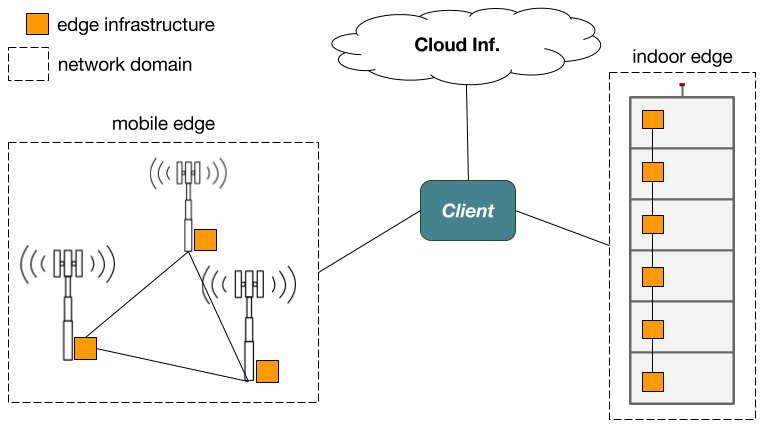
\includegraphics[width=0.51\textwidth]{figs/edge-heterogeneity.png}}
%	\captionsetup[subfigure]{width=0.43\textwidth}	
%	\hfill
%	\subfloat[The heterogeneity of different cloud and edge compute platforms and infrastructures abstracted as domains\label{fig:edge-domain-client}] {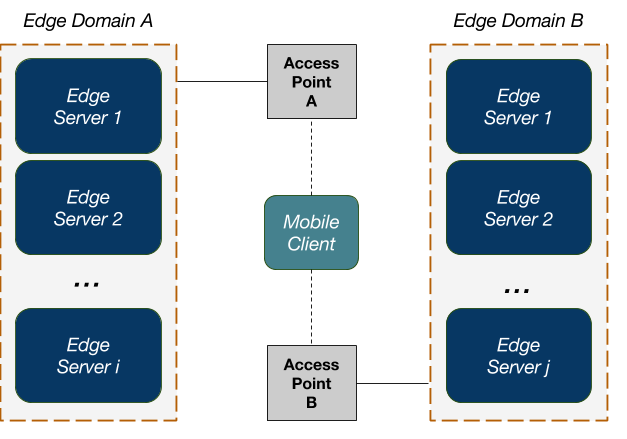
\includegraphics[width=0.43\textwidth]{figs/edge-domain-client.png}}
%	\hfill\null
%	\caption{Continuum heterogeneity}\label{fig:1}
%\end{figure}

%In addition, different kinds of edge infrastructure (e.g., more powerful servers or single board computers) or the same kind of edge infrastructure at different contexts (e.g., the number of clients in an area is too high in one region and low in another) may fit better with different policies for edge resources usage. 

%Client applications heterogeneity
%Client applications may significantly differ in terms of the QoS they require from services and providers. For example, connected vehicles (CV) may eventually rely on edge services for low-latency computation. A CV entering a given region for the first time is unlikely to be waiting until the edge servers covering that region become ready for providing the service the vehicle requires. Conversely, users of an augmented reality application could eventually wait for a setup time whenever the nearby edge \textit{domain}
%%
%~\footnote{From this point on, the term \textit{domain} is used to abstract whatever computational resources can be employed by different computing platforms (i.e., those used by cloud, mobile-edge, local-edge, and local). It is also implied that edge domains are accessible by clients through some (network) access point (Fig.~\ref{fig:edge-domain-client}).} 
%%
%is not ready. 
%%In both cases, low-latency is an important requirement. However, the later type of application could afford a setup delay which the first could not.
%Accordingly, the unified model should enable the co-existence of applications requiring different QoS levels (\stepcounter{req_count}\textbf{R\arabic{req_count}}); and the priority of the usage of computational resources from resource-constrained domains must be in accordance with the application category and its QoS requirements (\stepcounter{req_count}\textbf{R\arabic{req_count}}).

\subsubsection*{Efficiency}\label{sec:efficiency}

\stepcounter{req_count}

An important aspect is that of efficiency. In cloud computing, the infrastructure responsible for hosting and performing services is abstracted away from client applications through virtualization and more recently containerization technologies. In particular, the horizontal scalability provided by virtually unlimited cloud resources enables the optimization of cloud services availability by allowing elastic services to remain accessible and operational independently of the number of requests. ployed to each edge domain, even when there are no clients in the area being served. Such a high availability suits well with services covering either large or dense areas in which requests are always expected. In contrast, the fine grained nature of edge computing suggests the need of a different approach for the usage of its computational resources~\cite{GarrigaMendonca2017}.

%The elasticity of cloud datacenters is enabled by its horizontal scalability, in which virtual machines or containers can be instantiated in new virtually unlimited physical resources. 


%...in which backend applications are deployed to virtual machines and/or containers....

%A direct replication of cloud computing IaaS model with edge computing infrastructure would not be possible. 

First, because it is unlikely that a significant number of applications could be simultaneously hosted by edge servers using technologies such as virtualization and containerization. Even if containers can be allocated faster than virtual machines~\cite{Quatrocchi2016discrete}, at its best, a minimum amount of resources still needs to be allocated to always-deployed containers. Thus, the scalability of edge computing in terms of number of simultaneous services and clients would be reduced. Second, because it is unlikely that clients of services covering small areas shall always be present. To improve efficiency and scalability, the allocation of runtime resources to different services should be opportunistic and without minimum preallocation, unless justified otherwise (Req. \stepcounter{req_sub_count}\textbf{R\arabic{req_count}.\arabic{req_sub_count}}). Moreover, the fine-grained distribution of edge domains and their resource limitations also suggests that an a priori acquisition of different service artifacts to all domains would impose unnecessary burden. Even if storage is more abundant and cheaper resource than runtime resources like CPU and memory, a proactive and indiscriminate acquisition of service artifacts could compromise the scalability of edge computing. Accordingly, the acquisition of service artifacts should be opportunistic, unless justified otherwise (Req. \stepcounter{req_sub_count}\textbf{R\arabic{req_count}.\arabic{req_sub_count}}).

\subsubsection{Locality \& Context-Awareness}\label{sec:context-awareness}

\stepcounter{req_count}

In a fine grained distribution of edge computing, it is unlikely that different service providers will be able to coordinate and decide which one will serve a given client request. For instance, from inside a building with some local-edge domain accessible through Wi-Fi direct, a client may still be in contact with a mobile-edge accessible through 5G\footnote{Fifth generation of broadband cellular technology}. If both can provide the same services, but are unable to communicate and coordinate the allocation of the client request, it is up to the client to make the decision of which domain to use. Accordingly, clients should have the control over which service providers in the continuum should be used (Req. \stepcounter{req_sub_count}\textbf{R\arabic{req_count}.\arabic{req_sub_count}}). 

The discovery of finely distributed edge datacenters is another important aspect to be tackled. Today, networking protocols and technologies are the main responsible for allowing client applications to access cloud services in a transparent way. For this, clients access cloud services by means of well-known Internet names that are resolved by traffic managers and domain-name servers (DNS) technologies. The datacenters hosting cloud services are, at best, coarsely distributed among continents, countries, or broader regions. Conversely, finely distributed edge datacenters may be part of the local network infrastructure (e.g., domestic and office infrastructures). Such configuration requires that servers and services to be discoverable by clients (Req. \stepcounter{req_sub_count}\textbf{R\arabic{req_count}.\arabic{req_sub_count}}).


%In these cases, services names are mapped to either the servers hosting them or to intermediate components (e.g., traffic managers) responsible for transparently routing client requests to datacenters covering their area. 
%In contrast, in a , a similar transparency may not be possible. 



%Additionally, to allow services to be opportunistically deployed based on the awareness of clients in their coverage area, clients must advertise their requirements to service providers (Req. \stepcounter{req_sub_count}\textbf{R\arabic{req_count}.\arabic{req_sub_count}}).

%clients must be aware of alternative domains (Req. \stepcounter{req_sub_count}\textbf{R\arabic{req_count}.\arabic{req_sub_count}}); and 

%First, because 

%Second, because clients can switch from one network to the other at their discretion or make simultaneous use of different connections.

%Additionally, as mobile clients can enter or exit a given area, their connectivity with a given edge domain may be lost. The less time a mobile client remains connected to a domain, the lower the chances of loosing connection before it is still processing that client's request. Thus, if services are not currently available in one domain, the later should not proxy the request to another domain. Instead, clients should perform direct requests to the cloud instead of having their request forwarded by the edge domain itself.

%In particular, two scenarios of edge computing are possible: 1) edge servers are part of the telecommunications infrastructure (e.g., they are located at cellular base stations); 2) edge servers are part of conventional infrastructure  (e.g., they are located at malls, concert halls, stadiums, office buildings, parks, etc). 
%
%In the first kind of scenario, which correspond to MEC, networking technology could be employed to make the decision of using edge or cloud infrastructure transparent for the client. For instance, active components at the base stations could divert the traffic coming from clients connected to that base station to local edge servers whenever the requested services are available or to the cloud otherwise~\cite{MEC_ROUTING}. 
%
%Analogously, the second kind of scenario would require local network infrastructure components like access points and routers to actively divert the traffic from clients to edge servers in that location upon availability or to the cloud otherwise.
%
%In both cases, clients requests would be transparently handled by either edge or cloud servers, with infrastructure components responsible for taking the edge-or-cloud decision. However, in the event of both types of edge infrastructure to coexist, the client would have to participate of an edge-or-edge kind of decision.


%For instance, at a given moment, the  client device may decide to switch from the mobile-edge domain to the local-edge domain. 

%As such, whereas independent edge servers would not see each other, the client would be able to see them and decide which one suits it the best.

%In addition to the client participation in a edge-or-edge kind of decision, there is an argument in favor of giving the client also the responsibility for the edge-or-cloud type of decision: mobility. 


%\begin{figure}[tbp]
%	\centering
%	\captionsetup[subfigure]{width=0.5\textwidth}	
%	\null\hfill
%	\subfloat[Heterogeneus and indpendent types of edge domains (mobile and indoor) in range of communication with a client device\label{fig:edge-heterogeneity}]{ 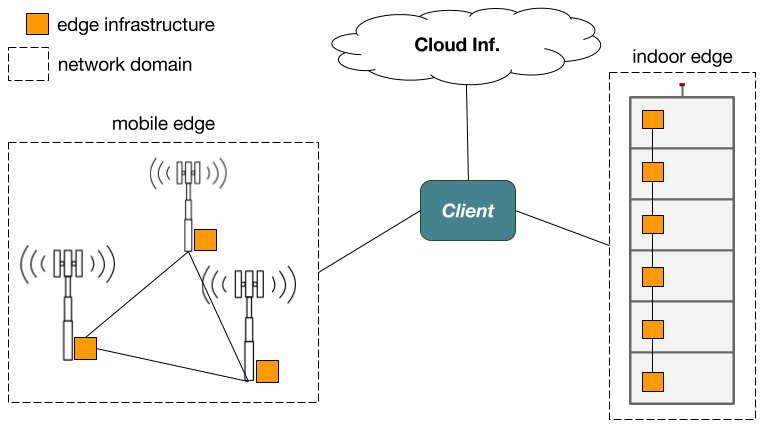
\includegraphics[width=0.5\textwidth]{figs/edge-heterogeneity.png}}
%	\captionsetup[subfigure]{width=0.45\textwidth}	
%	\hfill
%	\subfloat[In the case no edge service is available, client performs direct requests to the cloud and eliminate the dependency with intermediary edge domain infrastructure\label{fig:domain-selection}] {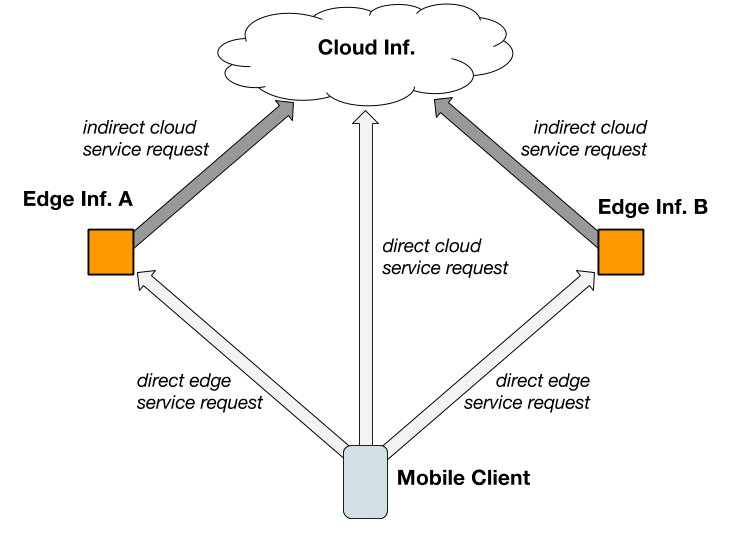
\includegraphics[width=0.45\textwidth]{figs/domain-selection.png}}
%	\hfill\null
%	\caption{Edge heterogeneity and client awareness}\label{fig:no-label-here}
%\end{figure}

%TODO: replace R2 with: Control over forwarding from edge to cloud. Soft vs. strong constraint. Soft = I can also run on cloud if needed. Strong = Never go to cloud.
	
\subsubsection{Automation and Encapsulation}

\stepcounter{req_count}

As a key aspect to realization of the computational continuum lies automation. First, because the multiplicity of finely distributed edge datacenters requires the self-managing of this infrastructure to avoid the burden and costs of manual human operation. Second, automation is needed to allow services to be seamlessly displaced from different parts of the continuum. Accordingly, automation should encompass the operational aspects of services life-cycle, including the allocation of resources for different services (Req. \stepcounter{req_sub_count}\textbf{R\arabic{req_count}.\arabic{req_sub_count}}) and the installation of services (Req. \stepcounter{req_sub_count}\textbf{R\arabic{req_count}.\arabic{req_sub_count}}). Finally, it should also encompass the choice of alternative domains by a client (Req. \stepcounter{req_sub_count}\textbf{R\arabic{req_count}.\arabic{req_sub_count}}).


%in the context of a shared platform 

%Following a serverless architecture, the application developer has control over the code they deploy into the infrastructure. 
%The model should be automated and transparent, where the developer is unaware of which infrastructure is using to run her applications. 

%In specific, the allocated resources should be scaled to zero where no servers are actually running when the application's function code is not used, and there is no cost to the user nor overload to the platform.


%Therefore, the management of computational resources must be automated and not depend on  manual intervention from human administrators (\textbf{R\arabic{req_count}}).


%Differently from classical \textit{on-premise} servers, edge should benefit from the automation and other characteristics of the A3-E model. As a result, local-edge servers can be seen as automated black boxes requiring no manual maintenance.	
	
%The fulfillment of the above requirements would leverage the potential of edge computing by optimizing the usage of its resources and consequently allowing a larger number of client applications to share the costs of edge infrastructure. Moreover, the resulting unified model would work as an extension of today's cloud IaaS/FaaS with the twofold purpose of enabling applications with low-latency requirements to rely on edge domains and to augment the computational power of mobile devices through mobile-to-edge computation offloading. Last but not least, the computing power of highly available and elastic cloud services would remain as an essential part of the continuum.
